\section{Evaluation}
\label{sec:Evaluation}
In this section, a quantitative evaluation of our system is presented on the entity-aspect dataset from Nanni et al.\cite{nanni2018entity}. We begin by presenting some research questions pertaining to three broad components of our system: Entity Salience, Entity Relatedness and Co-occurring entities, which our experiments aim to address(Section \ref{subsec:Research Questions}). We then describe our experimental settings (Section \ref{subsec:Evaluation Paradigm}), followed by the baselines (Section \ref{subsec:Baselines}). We end this section with a discussion of our experiments and results (Section \ref{subsec:Results}).

\subsection{Research Questions}
\label{subsec:Research Questions}

\begin{itemize}
\item[\textbf{RQ1}] Does entity salience affect the task? If yes, then to what extent?
\item[\textbf{RQ2}] Does entity relatedness affect the task? If yes, then to what extent? 
\item[\textbf{RQ3}] Is the frequency or relatedness of co-occurring entities a better indicator of a good aspect?
\item[\textbf{RQ4}] Can we use co-occurring entities to infer the correct entity aspect?
\item[\textbf{RQ5}] Does filtering out non-relevant co-occuring entities improve results when inferring the correct entity aspect?
\end{itemize}

\subsection{Evaluation Paradigm}
\label{subsec:Evaluation Paradigm}

\paragraph{\textbf{Datasets.}}
Due to the lack of other datasets in this area, we use the Entity Aspect Linking dataset from Nanni et al.\cite{nanni2018entity} to evaluate our methods. It consists of 201 entity mentions from Wikipedia along with their sentence, paragraph and section context and a list of candidate aspects for the mention.  We use the TREC Complex Answer Retrieval track \cite{dietz2018trec}\footnote{\url{http://trec-car.cs.unh.edu}} dataset as a source of passages when building the Entity Context Document in Section \ref{subsubsec:Co-occurring entities based features}. It consists of an entity linked corpus consisting of paragraphs from the entire English Wikipedia.

\paragraph{\textbf{Ground Truth.}} The dataset from Nanni et al. \cite{nanni2018entity} contains a ground truth file which maps a mention to the correct aspect. The TREC Complex Answer Retrieval track \cite{dietz2018trec} dataset contains both passage and entity ground truth data, however in our work, we do not need to use them. 

\paragraph{\textbf{Evaluation Metrics.}} We use Precision at 1 (P@1) and Mean Reciprocal Rank (MRR) as our evaluation metrics.

\paragraph{\textbf{Machine Learning.}}
We apply our methods to produce an aspect ranking for every entity mention. We then treat each ranking as a feature and perform 5-fold cross validation with a listwise learning-to-rank (L2R) method (Coordinate Ascent) optimized for Precision at 1 (P@1). We use RankLib\footnote{Dang, V. "The Lemur Project-Wiki-RankLib." Lemur Project,[Online]. Available: \url{http://sourceforge. net/p/lemur/wiki/RankLib}.} for this purpose. 


\subsection{Baselines}
\label{subsec:Baselines}

\textbf{Baseline 1: Nanni et al.} We re-implement all features from Nanni et al. \cite{nanni2018entity} and use a supervised combination of sentence, paragraph and section context features as our baselines. \\
\textbf{Baseline 2: Size.} We consider the length of each section (in number of tokens) and link the entity-mention to the longest. \\
%\textbf{Baseline 3: Content Overlap.} Overlap between the tokens in the sentence, paragraph and section context of the mention. \\
%\textbf{Baseline 4: Entity Overlap.} Overlap between the entities in the sentence, paragraph and section context of the mention. \\

\subsection{Results}
\label{subsec:Results}
The most interesting results are presented in Table \ref{tab:Results}. Due to space constraints other results were moved to the online appendix for this paper. Below, we discuss each of the research questions presented in Section \ref{subsec:Research Questions}.
%Below, we discuss results from our experiments with respect to the three broad components of our system: entity salience, entity relatedness and co-occurring entities, and answer the research questions presented in Section \ref{subsec:Research Questions}.


\begin{figure}
    \centering
    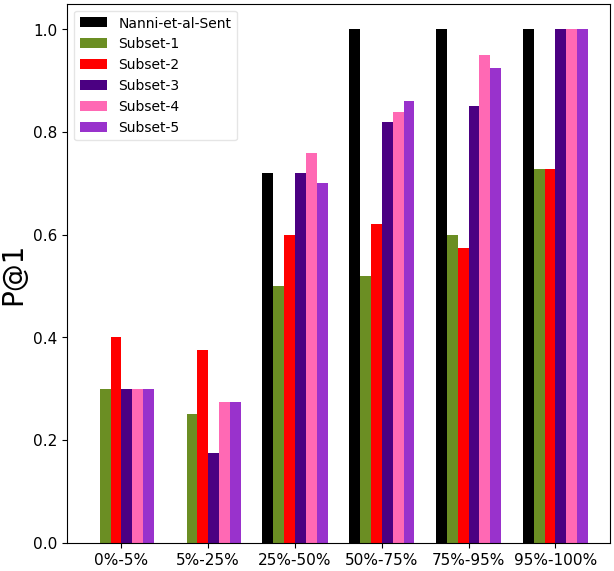
\includegraphics [scale=0.5]{plot-cropped.png}
    \caption{Difficulty-test for P@1, comparing Nanni et al.(Sentence) to various L2R systems.}
    \label{fig:difficulty-plot}
\end{figure}


\begin{table}[t]
    \caption{Performance with standard error of individual features and combined with L2R, including subsets/ablations.}
    \label{tab:Results}
    \scalebox{0.9}{
    \begin{tabular}{@{}lllll@{}}
        \toprule
        Method & 
       P@1 &
        MRR \\ 
        
        \midrule
        
     
      
     
      Nanni et al. (Sentence)&  
      0.67$\pm$0.03&
      0.79$\pm$0.02
      \\
      
      
    
      Nanni et al. (Paragraph)&  
      0.64$\pm$0.03&
      0.78$\pm$0.03
      \\
      
      Nanni et al. (Section)&  
      0.53$\pm$0.03&
      0.71$\pm$0.03
      \\
      
     
      Size &
      0.39$\pm$0.03&
      0.60$\pm$0.03
      \\
      
      \midrule
      
     
    Sal-EM   &   
      0.19$\pm$0.03 &
      0.46$\pm$0.03
      \\
      
      
      
      SEC (Sentence)  &    
      0.23$\pm$0.03 &
      0.53$\pm$0.03
      \\
      
      
      AEC (Sentence)   &    
      0.51$\pm$0.03 &
      0.70$\pm$0.03
      \\
       \midrule
      
     
      SF-Dist (Sentence)   &    
      0.54$\pm$0.03 &
      0.72$\pm$0.03
      \\
      
     
      WF-Dist (Sentence)  &    
      0.49$\pm$0.03 &
      0.67$\pm$0.03
      \\
      
      
      Rel-Dist (Sentence)  &    
      0.43$\pm$0.03 &
     0.62$\pm$0.03
      \\
       \midrule
      
    
      SF-Dist-ECD   &    
      0.35$\pm$0.03 &
      0.59$\pm$0.03
      \\
      
      
      Rel-Dist-ECD  &    
      0.36$\pm$0.03 &
      0.60$\pm$0.03
      \\
      
     
      RS-Asp-Freq-ECD (LMJM + RM1)  &     
      0.35$\pm$0.03 &
      0.59$\pm$0.03
      \\
      
       
      RS-Asp-Rel-ECD (LMJM + RM1) &     
      0.40$\pm$0.03 &
      0.60$\pm$0.03
      \\
       \midrule
      
      
      Rel-Dist-Wiki  &    
      0.37$\pm$0.03 &
      0.60$\pm$0.03
      \\
      
      
       
      RS-Asp-Rel-Wiki (BM25 + RM3)  &     
      0.39$\pm$0.03 &
      0.61$\pm$0.03
      \\
      \midrule
      
       Subset-1 (Only Relatedness) &
      0.48$\pm$0.03 &
      0.68$\pm$0.03
      \\
      
      
      Subset-2 (Only Salience) &
      0.59$\pm$0.03 &
      0.72$\pm$0.03
      \\
      
       Subset-3 (Rel. + Lex. + Sem.) &
      0.66$\pm$0.03 &
      0.78$\pm$0.03
      \\
      
       Subset-4 (Sal + Lex. + Sem.) &
      
      0.72$\pm$0.03 &
      0.82$\pm$0.03
      \\
      
      
      Subset-5 (Sal. + Rel. + Lex. + Sem.) &
      0.70$\pm$0.03 &
      0.81$\pm$0.03
      \\
     
      
      

     
      
       \bottomrule
    \end{tabular}
    }
\end{table}


%\subsubsection{Entity Salience}
%\label{subsubsec:Entity Salience}
\textbf{RQ1: Entity Salience.}
%\paragraph{\textbf{Observations.}}
We observe from Table \ref{tab:Results} that a supervised combination of all salience features (Subset-2) outperforms 2 of the 4 baselines, whereas a combination of all salience features with the lexical and semantic features (Subset-4) outperforms all baselines. However, considering all entities (salient and non-salient) in the context (AEC Sentence) performs better than considering only the salient entities (SEC Sentence). We also find that in Subset-2, learning-to-rank always places maximum weight on the AEC methods.
%\paragraph{\textbf{Discussions.}}
These observations show the effectiveness of using salience. However, they also indicate that considering non-salient entities together with the salient ones help improve performance. We manually confirmed that SWAT correctly identifies salient entities in text. However, SWAT returns more empty results when asked for only salient entities than when asked for all (salient or otherwise) entities. For example, using the sentence context of an entity mention, it returns an empty result for 100 of the 201 entity mentions when asked for only the salient entities and 13 of 201 entity mentions when asked for all  entities. This shows the limitations in SWAT and why the results obtained using \textit{SEC (Sentence)} is lower than \textit{AEC (Sentence)}.  Our intuition is that the other entities, although non-salient, have some inherent semantic meaning and hence considering them together with the salient entities helps the task. %This is the case for the paragraph and section contexts too but we do not show the results here due to space constraints. 

To investigate the extent to which salience helps, we divide the entity mentions  into different levels of difficulty according to the performance (P@1) of the \textit{Nanni et al. (Sentence)} method, with the 5\% most difficult queries fo
r this method to the left and the 5\% easiest ones to the right, and compare the performance with the \textit{Subset-4}. The results are shown in Figure \ref{fig:difficulty-plot}. We observe that whenever it is difficult to perform the task using \textit{Nanni et al. (Sentence)}, entity salience supports our L2R system (Subset-2 and Subset-4).

\textbf{Conclusions.}
Entity salience does indeed affect the task positively by learning information which is complimentary to the lexical and semantic features. However, the limitations of SWAT hinder the performance of a system using it.

%We are able to outperform all the baselines with the help of salience and we see that salience helps to boost performance when the queries get difficult. However, SWAT is still limited in its salience detection and this hinders the performance of a system using it. 

\textbf{RQ2: Entity Relatedness.}
%\subsubsection{Entity Relatedness}
%\label{subsubsec:Entity Relatedness}
%\paragraph{\textbf{Observations.}}
We observe from Table \ref{tab:Results} that a supervised combination of all relatedness features (Subset-1) does not perform very well on its own, doing better than only one baseline (Size). However, a combination of relatedness features with the lexical and semantic features (Subset-3) does significantly better than 3 of the 4 baselines. Moreover, a combination of salience and relatedness features with the lexical and semantic features outperforms all baselines. 
%\paragraph{\textbf{Discussions.}}
These observations indicate that entity relatedness does indeed affect the task positively. However, salience is more informative than relatedness as is evident from the superior performance of Subset-2 over Subset-1 and Subset-4 over Subset-3. On further investigation, we found that WAT finds many false positives and false negatives. For example, given the entity list consisting of  \textit{World War I}, \textit{Vietnam War} and \textit{France}, it predicts that \textit{World War I} is related to \textit{Vietnam War} (false positive) but  unrelated to \textit{France} (false negative). This is because WAT does not take
the query or the context of the entity into account but makes predictions based on certain graph-based features such as number of inlinks and outlinks to and from a particular entity node in a knowledge graph. Moreover, from the difficulty plot in Figure \ref{fig:difficulty-plot}, we observe that whenever it is difficult to perform the task using \textit{Nanni et al. (Sentence)}, entity relatedness supports our L2R system (Subset-3 and Subset-5).


\textbf{Conclusions.}
Although relatedness of entities by itself may not perform very well, a supervised combination with lexical and semantic features improves performance over several baselines. However, the limitations of WAT hinder the performance of a system using it.

%considering relatedness features in combination with some lexical and semantic features can help the task. However, WAT is limited in its entity relatedness system where it finds many false positives and false negatives.

\textbf{RQ3: Frequency vs Relatedness.}
%\subsubsection{Co-occurring Entities}
%\label{Co-occurring Entities}
From Table \ref{tab:Results}, we observe that ranking aspects using \textit{SF-Dist (Sentence)} outperforms \textit{WF-Dist (Sentence)}, which in turn outperforms \textit{Rel-Dist (Sentence)}). Moreover, \textit{RS-Asp-Freq-ECD} outperforms \textit{RS-Asp-Rel-ECD}. We also find that when L2R is trained on all relatedness features (Subset-1), it places more weight on the features using frequency distribution those using relatedness. These observations indicate that using the frequency of co-occurring entities is more informative than the relatedness. To investigate this further, we evaluate the quality of the intermediate entity rankings produced by using the frequency and relatedness of entities in Sections \ref{subsubsec:Entity relatedness based features}(1) and \ref{subsubsec:Entity relatedness based features}(3) by defining all entities in an aspect as relevant for the aspect. We find that the entity rankings obtained using frequency distribution are indeed better (in terms of
Mean Average Precision (MAP)) than those obtained using relatedness. For example, entity ranking obtained using section context and frequency distribution has $\text{MAP}=0.13$ whereas that obtained using relatedness has $\text{MAP}=0.04$. 

\textbf{Conclusions.} Using frequency of co-occurring entities is better than using relatedness because most frequently co-occurring entities are also related but most related entities do not frequently co-occur.
